%!TEX root = ../main.tex
\section{Introduction} 
\label{sec:intro}
Data quality is one of the most significant problems in data management, among which mislabels are a common dirty data type that could directly lead to  low-quality data analysis  and misleading business decisions. Labels are always large-scale and error-prone because they may be crowdsourced from non-experts or collected from web annotations, so it is inevitable to use automatic methods to detect mislabels. However, existing mislabel detection approaches suffer from fair accuracy.


\stitle{Existing Solutions.} Traditional methods~\cite{} rely on the data locality to detect mislabels. For example, in order to whether the label of an instance in a dataset is correct, the typical KNN method~\cite{} checks its neighbors, and if they have inconsistent labels, the instance tends to be mislabeled, otherwise it is a clean one. This type of methods has low detection accuracy because they just consider the local neighbors of each instance rather than the entire dataset. Therefore, to improve the accuracy, machine learning (ML) models are incorporated to help mislabel detection~\cite{} because intuitively,  mislabels definitely have impact on the supervised model training. For instances, ensemble-based methods~\cite{} involve multiple models to train on the entire dataset and check the consistency of the prediction results from these models for each instance. Cleanlab~\cite{} utilizes confident learning to estimate the joint distribution of mislabels and correct labels. This line of methods can capture the entire data distribution of the dataset through ML and avoid the data locality problem. However, the accuracy is still not high because they learn the distribution from both the incorrect and correct labels. In this way the model has already fitted on the dirty data, and thus the learned distribution is not accurate, leading to inaccurate prediction results.


\stitle{Challenge.} As discussed above, to pursue high accuracy of mislabel detection, we have to consider the data distribution of the entire dataset rather than the locality. In terms of using ML to capture the distribution, it is challenging to eliminate the impact of mislabels on the learned distribution. Ideally, if we know the distribution learned from all clean instances, we can easily use it to detect the dirty ones, but unfortunately, we cannot know it in advance.

Based on the challenge, we have the following observation and proposed methods.


%\stitle{Problem.}
%Our main research question in this paper is how to \textit{detect mislabeled data in the large training set which will be used for the downstream meachine learning model} and filter it to improve the data quality of training set. A positive answer to this question is crucial as it can help machine learning model to learn more correctly about the distribution of the training set, so as to obtain better model performance.


\stitle{Observation.} Since it is inappropriate to detect mislabels after training because the model has already fitted the dirty data. We consider whether we can leverage the metadata during (or at the beginning of) training to help detect mislabels. The high level intuition is that this strategy clearly avoids data locality because all instances participate in training, while it can also capture the entire data distribution to a certain degree before the model fits dirty instances. 

\stitle{Our proposal.}
Our main idea is to find out the instance in the training set which is labeled incorrectly.
More specifically,% \nan{Add more details later.}

\stitle{Contributions.}
Our contributions are summarized as follows:


\begin{figure*}
	\centering
	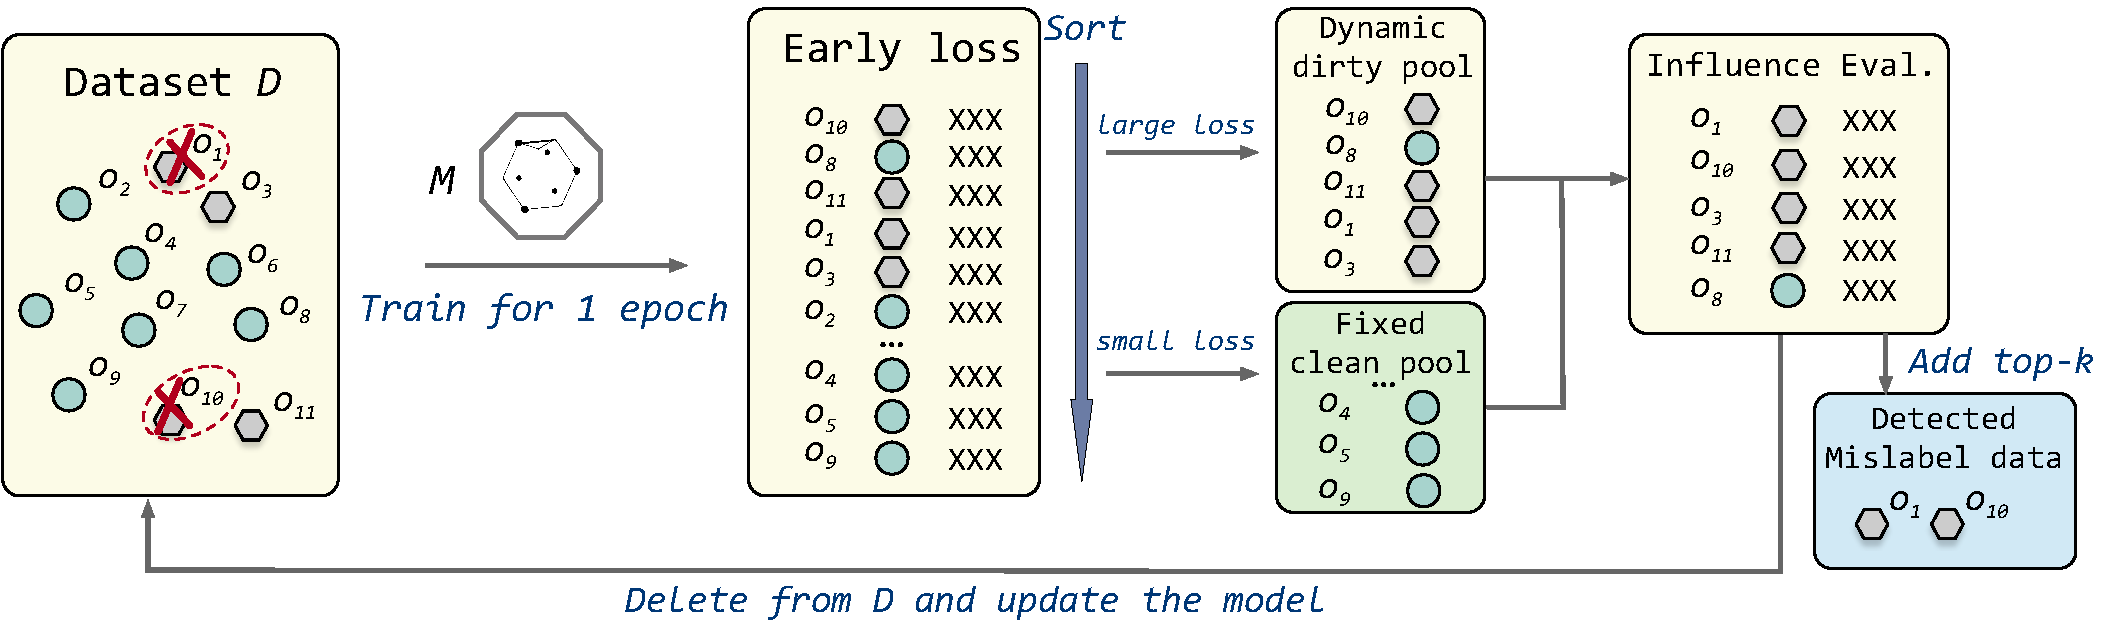
\includegraphics[width=\textwidth]{figures/framework}
	\caption{\sys Framework}
	\label{fig:framework}
\end{figure*}


\be
	\item 
	\item 
	%\item \nan{If we can have a good summary of experiments, we can either add here or use a ``stitle'' section to highlight the empirical findings.}
\ee



% \begin{figure*}
%	\centering
%	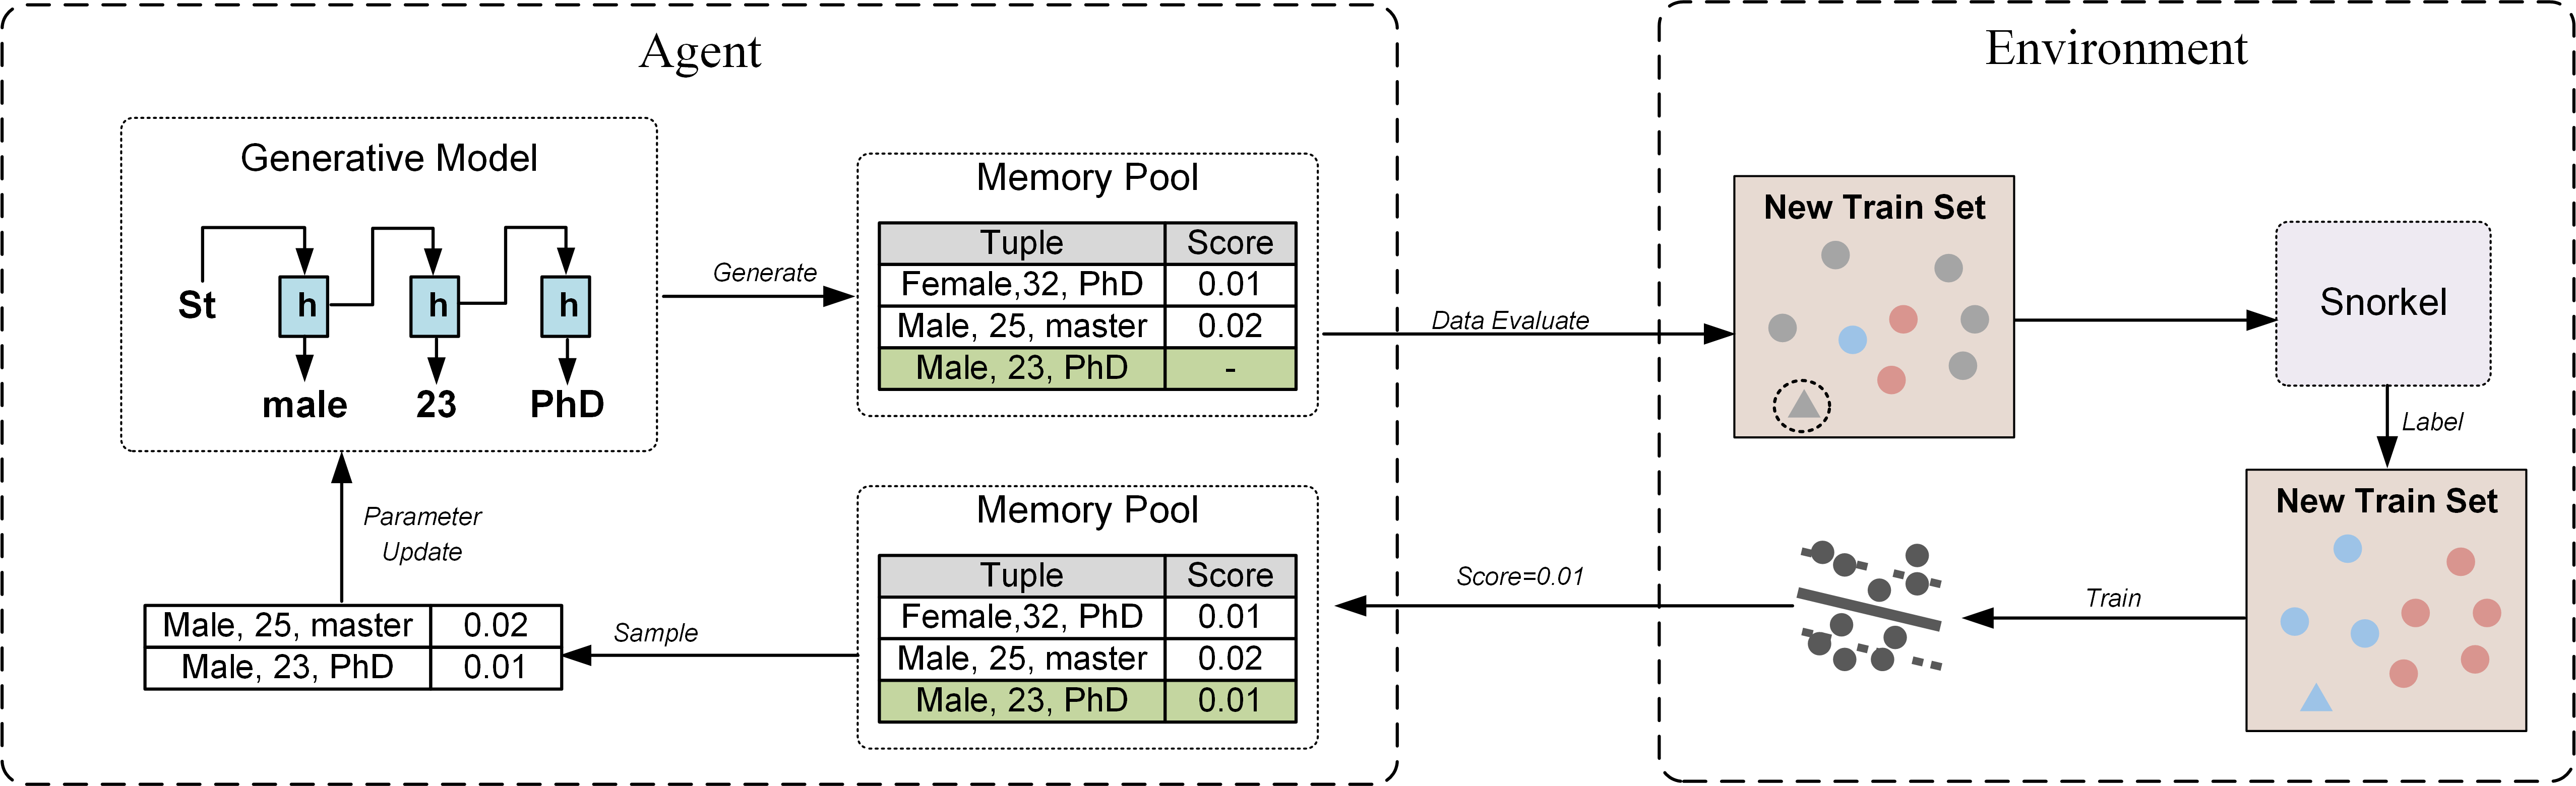
\includegraphics[width=\textwidth]{figures/overview.png}
%	\caption{Framework}
%	\label{fig:framework}
% \end{figure*}

% \begin{itemize}
% 	\item The difference between traditional data generation and ours (for ML model).
% 	\item (Challenge) The key challenges of this problem: learn the generative model from feedback; how to evaluate generated tuples.
% \end{itemize}